% options:
% thesis=B bachelor's thesis
% thesis=M master's thesis
% czech thesis in Czech language
% english thesis in English language
% hidelinks remove colour boxes around hyperlinks

\documentclass[thesis=B,czech]{FITthesis}[2013/10/20]

\usepackage[utf8]{inputenc} % LaTeX source encoded as UTF-8

\usepackage{graphicx} %graphics files inclusion
% \usepackage{amsmath} %advanced maths
% \usepackage{amssymb} %additional math symbols

\usepackage{dirtree} %directory tree visualisation

\usepackage{float}
\usepackage{wrapfig}
\usepackage{caption}
\usepackage{listings}

\usepackage{courier}

\lstset{basicstyle=\footnotesize\ttfamily,breaklines=true}
\lstset{framextopmargin=50pt}

% % list of acronyms
% \usepackage[acronym,nonumberlist,toc,numberedsection=autolabel]{glossaries}
% \iflanguage{czech}{\renewcommand*{\acronymname}{Seznam pou{\v z}it{\' y}ch zkratek}}{}
% \makeglossaries

\newcommand{\tg}{\mathop{\mathrm{tg}}} %cesky tangens
\newcommand{\cotg}{\mathop{\mathrm{cotg}}} %cesky cotangens

% % % % % % % % % % % % % % % % % % % % % % % % % % % % % % 
% ODTUD DAL VSE ZMENTE
% % % % % % % % % % % % % % % % % % % % % % % % % % % % % % 

\department{Katedra \ldots (Softwarového inženýrství)}
\title{Evidence potravin v OS Android}
\authorGN{Filip} %(křestní) jméno (jména) autora
\authorFN{Kofroň} %příjmení autora
\authorWithDegrees{Filip Kofroň} %jméno autora včetně současných akademických titulů
\supervisor{Ing. Jiří Hunka}
\acknowledgements{Doplňte, máte-li komu a za co děkovat. V~opačném případě úplně odstraňte tento příkaz.}
\abstractCS{Tato bakalářská práce seznamuje čtenáře s globálním problémem plýtvání potravin. Popisuje možné řešení v podobě mobilní aplikace od jeho analýzy, návrhu pro jednoduchost použití a efektivitu, až po implementaci mobilního klienta v prostředí OS Android a serverovou částí využívající svobodný software následovanou testováním. Práce dále hodnotí výsledné řešení a nabízí pohled do jeho budoucnosti s případnými vylepšeními, které přinesla odezva při nasazení aplikace u skutečných uživatelů.}
\abstractEN{Sem doplňte ekvivalent abstraktu Vaší práce v~angličtině.}
\placeForDeclarationOfAuthenticity{V~Praze}
\declarationOfAuthenticityOption{1} %volba Prohlášení
\keywordsCS{Nahraďte seznamem klíčových slov v češtině oddělených čárkou.}
\keywordsEN{Nahraďte seznamem klíčových slov v angličtině oddělených čárkou.}

\begin{document}

% \newacronym{CVUT}{{\v C}VUT}{{\v C}esk{\' e} vysok{\' e} u{\v c}en{\' i} technick{\' e} v Praze}
% \newacronym{FIT}{FIT}{Fakulta informa{\v c}n{\' i}ch technologi{\' i}}

\begin{introduction}

Plýtvání potravin je celosvětový problém, který má přímé následky v plýtvání zdrojů k výrobě potravin, lidského času a sil. Tato činnost je pro mnohé výrobce a zprostředkovatele potravin peněžně výnosná, avšak pro samotnou přírodu včetně fauny a flóry zajisté ne. K chovu zvěře jsou nutné plodiny. Pro růst plodin je třeba prostor, který musíme zabrat na úkor ostatních rostlin a živočichů. Dle British Institution of Mechanical Engineers (IME) byla v roce 2013 odhadnuta skutečnost, že polovinou veškerých potravin na světě je plýtváno~\cite{fakta}.

Během posledních let vzniklo několik projektů, které se různými způsoby snaží tento problém řešit. Jsou to například způsoby domluvy různých lidí o nespotřebovaných potravinách, kdy lidé nabízí co mají navíc a za jiných okolností by vyhodili. Ostatní se mohou domluvit a jídlo si bezplatně či za výhodnou cenu převzít. Tento způsob používa mnoho webovch i mobilních aplikací.

Cílem této práce je vytvořit mobilní aplikaci, která pomůže uživatelům zabránit plýtvání potravin a nabídne jednoduché a rychlé rozhraní, díky kterému bude na uživatele kladena minímální časová náročnost.

V rozvinutých zemích po celém světě je dnes již dostatek potravin a jejich ceny nejsou pro běžné občany likvidační, jak je tomu naopak v některých rozvojových zemích. Přesto se však mnozí lidé snaží ušetřit jejich jmění a nakupovat co nejlevněji. To ovšem například znamená nakupování velkého množství aktuálně cenově výhodných potravin. Takové množství potravin se nemusí vždy podařit včas spotřebovat a lidem tak zůstanou prošlé potraviny, které buď dodatečně spotřebují nebo, pokud si nejsou jistí možnou závadností, potraviny vyhodí do odpadu.

Chytré mobilní telefony vlastní dnes již dostatek lidí na to, aby bylo možné docílit řešení tohoto problému právě skrze mobilní aplikaci. Jelikož je spousta potravin vyhazována do odpadu jen kvůli své opomenuté trvanlivosti, nabízí se řešení v podobě evidence potravin, která uživateli nabídne přehled o trvanlivosti jeho potravin a upozorní ho, pokud nějakým potravinám již trvanlivost skončí, či pokud se tak stane v blízké době.

V této práci popisuji vývoj mobilní aplikace od analýzy až po zhodnocení rozšíření její implementace. Práce využívá znalosti získané během mého studia z předmětů týkajících se algoritmizace, databázových systémů a počítačových sítí.

\end{introduction}

\chapter{Analýza}

Process vývoje musí projít několika následujícími fázemi, při kterých se analyzují všechny aspekty aplikace, které jsou potřeba při návrhu, finalní verifikaci výsledné implementace a jejím testovánim. 

Důraz analýzy je kladen především na potřeby uživatelů, neboť je nutné zaručit minimální nutnou funkcionalitu, která výrazně ovlivní náročnost rozhraní pro pochopení použití i jeho rychlost.

\section{Analýza konkurence}

Tato sekce popisuje aplikace, které více či méně konkurují výsledné aplikaci této práce a snaží se dále popsat jejich vlastnosti. Na konci sekce lze nalézt souhrn, který hodnotí všechny dosavadní řešení a jejich hlavní nedostatky. Informace z této sekce jsou velice důležité pro finální aplikaci. Můžou velice pomoci při hledání cesty k ještě lepšímu řešení než kterými jsou ty konkurenční. Takto lze posbírat důležité poznatky o jejich kladech i záporech, které vyplynou z vlastního otestování (pokud to bude možné) na následujícím seznamu zařízeních, které má autor k dispozici:
\begin{itemize}
  \item{Nexus 7, Android 4.4.2}
  \item{HTC Evo 3D, Android 2.3.3}
  \item{Vodafone 845 (Huawei U8120), Android 2.3.4}
\end{itemize}

V počátku tvorby této práce a implementací aplikace nebylo příliš mnoho konkurenčních aplikací k naleznutí. Jak se však později ukázalo, vzniklo a rozšířilo se během následujících činností několik dalších aplikací, které jen s maálo rozdíly splňují požadavky aplikace výsledkem této práce.

Tato část byla zprvu velice krátka, neboť jediné bližší aplikace neposkytovali vhodné srovnání ani zisk vhodných informací. V závěru jsem však usoudil, že některé tyto aplikace zaslouží zanalyzování a poskytnou tak čtenáři jistý nadhled nad daným tématem i v průběhu následujícího čtení. Dalším důvodem jejich zmiňky je autorovo zmýlení v jejich existenci v počátku, jelikož aplikace byly nedávno uvedené a nebylo dostatek vodítek k jejich naleznutí.

\subsection{Best before}

Aplikace Best Before je zdarma dostupná jak pro zařízení s iOS, tak pro zařízení s OS Android. Na první pohled je aplikace totožná na obou platformách. Při bližším zkoumání verze pro OS Android však bylo zjištěno, že aplikace využívá čisté prvky OS Android v částech jako jsou dialogy a některé běžné komponenty. Toto vytváří silný kontrast v rozhraní, který nemusí být pro uživatele OS Android příjemný přesto, že aplikace je jinak po stránce stylu více než na dobré úrovni.

Samotná funkcionalita aplikace je omezena a čistě přizpůsobena svému účelu. Aplikace disponuje seznamem potravin seřazeným v pořadí, v jakém jednotlivým potravinám vypřší spotřební lhůta. Přidání potraviny do aplikace lze tlačítkem v horním pravém rohu, které při stisku zobrazí jendoduchý formulář, ve kterém lze nastavit obrázek potraviny, název, místo uložení a z dialogu vybrat datum spotřeby.Nelze však zadat již existující potravinu a pokud uživatel zadává více potravin, může takto ztrávit poměrně dlouhou dobu.

Z vlastního testování však byly zjištěny zásadní nedostatky v ošetření různách chyb a stabilitě. Na žádném z použitých zařízení aplikace nebylo možné přidat obrázek potraviny, a při ukládání potraviny došlo při každém k pokusu k pádu, potravina se ve 4 z 5ti pokusů přidala, v jednom došlo ke kompletnímu smazání všech ostatních potravin. Aplikace byla tuďíž nepoužitelná. Z hodnocení na Google Play Store ~\cite{play_store} vyplývá, že někteřým uživatelům aplikace funguje bez problému, jiní naopak hlásí stejné problémy. Celkové hodnocení aplikace na Play Store se v rozsahu 1 až 5 umísťilo na hodnotě 3.9. Vzhledem k použitelnosti je tato hodnota spíše překvapivá.

Ve výsledku lze z této aplikace převzít zejména pozitivní přístup uživatelů k hezky nastylovanému rozhraní, které se zdá být jediným důvodem nadprůměrného hodnocení. Ačkoliv je toto pouze autorův názor, pro ověření by však bylo třeba širšího testování mezi různými uživateli, které ale je příliš časově náročné.

\subsection{Food Safe}

Další aplikací určenou pro Android OS je Food Safe ????, která se objevila na Play Store teprve nedávno, v době psaní tohoto textu přibližne 20 dní. Aplikace představuje přímou konkurenci aplikaci této práce. Informace o této aplikaci byly získány pouze z Play Store z toho důvodu, že nebylo možné nainstalovat aplikaci na žádné ze zařízení, které byly k dispozici při jejím testování v této práci. 

Aplikace není dostupná zadarmo. Je třeba ji zakoupit za částku, která v době psaní tohoto textu činí 20,40 Kč.

U této aplikace lze zaznamenávat potraviny pomocí jména a datumu spotřeby. Aplikace zdá se nabízí i možnost skenování čárových kódů, z hodnocení Play Store je ale zřejmé, že aplikace získává informace o potravinách od uživatelů a zaznamenává je do externí databáze. První uživatelé tedy budou nuceni zadávat ručně detaily všech jednotlivých potravin.

\subsection{Love Food Hate Waste}

Stejně jako aplikace Best Before je tato ve verzích pro iOS i Android OS. Rozhraní aplikace je témeř identické v obou verzích, používá styl a prvky obvyklé pouze pro iOS. Vzhled dává velmi dobrý dojem 
o aplikaci.

Nabízená funkcionalita zahrnuje:
\begin{itemize}
  \item{Recepty}
  \item{Množstevní plán}
  \item{Jídelníček}
  \item{Kuchyň - inventář potravin}
  \item{Nákupní lístek}
\end{itemize}

Z popisu aplikace není dostatek informací o jejich skutečné použitelnosti, z hodnocení uživatelů je ale patrné, že aplikace má mnoho nedostatků, kterými jsou nejčastěji omezení počtu kategorií jídel, zbytečně zobrazené kategorie způsobující nepřehlednost a vysoká nestabilita. Všechny tyto nedostaky vedli uživatele Play Store k celkovému hodnocení 2.5, tedy průměrnou hodnotu.

\subsection{Souhrn analýzy konkurence}

Ze všech výše uvedených aplikací je nejvíce podobná aplikaci této práce aplikace Food Safe. Nabízí možnosti, které usnadňují evidenci potravin, nenutí uživatele zadávat zbytečné informace a sbírá již zadaná data uživateli, aby je mohli použít i ostatní uživatelé. Přesto, že tato aplikace je velice podobná, aplikace této práce má snahu přinést ještě jednodušší způsob zadávání potravin, jejich společné sdílení a pokusit se disponovat více informacemi o potravinách, které do aplikace ještě žádný uživatel nezadal a umožnit takto jednodušší a především rychlejší zadání nové potraviny.

Nejzajímavější nápad aplikace Food Safe je bezesporu možnost načíst čárový kód. Autor si takto troufá tvrdit nejen proto, že informace o čárových kódech jsou dostupné volně na internetu, jak bude dále popsáno, ale také proto, že naprostá většina potravin, které lze koupit v běžných řetezcích, obsahují tyto čárové kódy, které jsou pro ně unikátní.

\section{Cílová skupina uživatelů}

Nepředpokládá se, že by se tato aplikace používala široce napřiklad v restauračních a jiných zařízeních disponujících závodními kuchyněmi, kterými prochází mnoho potravin a mobilní telefon pro tuto skupinu uživatelů nebude příliš pohodlný. Přesto však může aplikace stačit nějakému malému podniku, pokud si chce vést jednoduchou evidenci, jen aby předešel plýtvání, které by pro menší kapitál mohl znamenat veliký problém.

Autor však shledal nutnost aplikaci umožnit používat jakémukoliv členu rodiny či domácnosti. Je to zejména proto, aby mohl kdokoliv z rodiny použít rodinný účet a nově zakoupenou potravinu nebo právě spotřebovanou okamžitě přidat do aplikace, respektive odstranit. Nejen pro tento účel, ale i pro výše zmíněné sdílení informací o potravinách bude nutné, aby aplikace disponovala externím úložištěm dat.

Pro širší skupinu použití je vhodné u potravin evidovat i jejich jeden nebo více obrázků, které mohou vhodným způsobem odlišit jednotlivé potraviny i například pro lidi, kteří mají problém přečíst název potraviny, jejíž obrázek však rozpoznají jednodušeji. Autor nepředpokládá, že by tyto cílové skupiny potraviny přímo zadávali, a proto není nutné řešit problém zadání datumu spotřeby i pro tyto uživatele.

\clearpage

\section{Analýza požadavků}

Jako základ dalšího postupu aplikace je seznam jejích požadavků. Je třeba shrnout několik základních znalostí okolo problému, kterému se tato aplikace snaží nalézt řešení.

Prvním aspektem aplikace jako řešení je její rozšíření. Aby aplikace dosáhla k většině uživatelů a stala se tak efektivni, je zapotřebí zvolit takovou platformu, kterou používa nejvíce lidí. Z různých internetových zdrojů lze nalézt, že nejrozšířenější platforma na mobilních telefonech. Protože u žádného z těchto zdrojů nebylo možné zajistit autentičnost, byla k této práci vypracován krátký dotazník, na který odpovědělo 31 lidí. Cílem tohoto dotazníku bylo nalézt zajímavé informace, které pomůžou při výběru cílové platformy, a další informace pomáhající při volbě funkcionality. Výsledek rozšíření platforem mezi dotázanými lze nalézt na obrázku ~\ref{fig:SurveyOS}.

\begin{figure}[H]
  \centering
  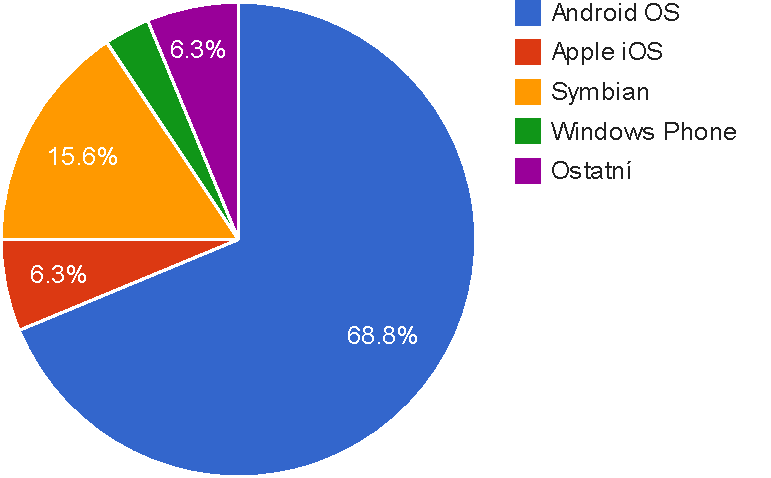
\includegraphics[scale=0.8]{charts/survey_os}
  \caption{Rozšíření mobilních platforem}
  \label{fig:SurveyOS}
\end{figure}

Výběr cílové platformy je tedy jistý. Čtenář může jistě dohledat další průzkumy rozšíření platforem, které jsou více či méně rozdílné, avšak všechny poukazují na fakt, že OS Android je nejrozšířenější, dává si za cíl tato práce poskytnout řešení pro tuto platformu. Protože budoucnost této aplikace může přinést rozšíření i na více platforem, je nutné zajistit, aby společené úložiště dat aplikace bylo možné použít i pro jinou platformu. Toto zajistí multiplatformní protokol.

Vzhledem k tomu, že většina potravin disponuje čárovým kódem a k tomuto kódu můžou být dohledány informace o zboží, které identifikuje, lze aplikaci vybavit čtečkou čárových kódu, která usnadní manuální zadávání názvu či tohoto kódu. Aby tato informace nebyla jen tak nadhozena, byla do dotazníku přidána další sekce. Na obrázku ~\ref{fig:SurveyScan} lze pozorovat poměr mezi dotázanými, kteří by využili možnosti zadávat jídlo pomocí čtečky a těmi, kteří by toho nevyužili.

\begin{figure}[H]
  \centering
  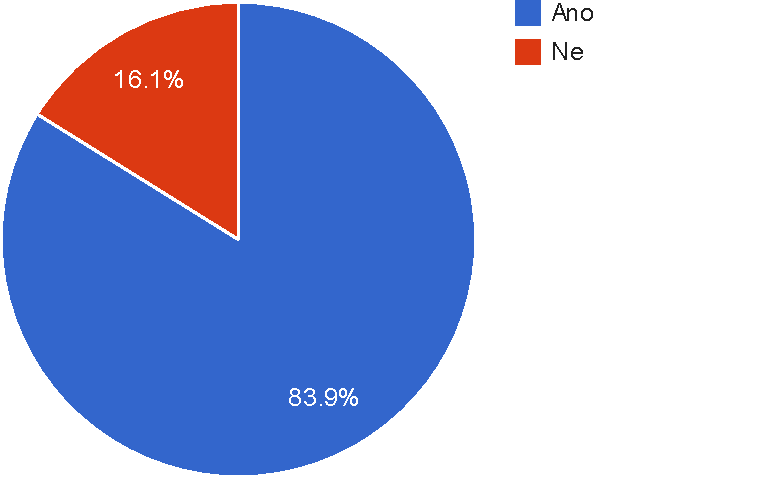
\includegraphics[scale=0.8]{charts/survey_scan}
  \caption{Žádanost zadávání potravin pomocí čtečky čárového kódu}
  \label{fig:SurveyScan}
\end{figure}

Funkční požadavky této aplikace, které plynou z daného problému a výše uvedených výsledků dotazníku jsou:

\begin{itemize}
  \item přidávání nových potravin
  \item sdílení známých potravin
  \item specifikace běžné doby spotřeby potraviny
  \item zaznamenání fotografie potraviny
  \item zaznamenávání potravin do inventáře
  \item odebírání potravin z intentáře
  \item zaznamenání data spotřeby
  \item hledání potraviny pomocí čárového kódu nebo názvu
  \item čtení čárového kódu pomocí kamery mobilního telefonu
  \item upozornění na jídlo, jehož spotřební doba se ocitla v krátkém intervalu mezi koncem, či jehož spotřební doba již uplynula
  \item nastavení intervalu pro upozornění o spotřebě, který je rozdílem doby spotřeby potraviny a aktuálního data
  \item získávání informací o neznámých potravinách z otevřené databáze čárových kódů
\end{itemize}

Čárové kódy na obalech potravin bývají různého formátu. Obecně se v na obalech objevují kódy typu GTIN, které pokrývají většinu mezinárodně rozšířených. Kódy jsou číselné a mohou nabývat délky od 8 do 14ti číslic. Kratší kódy lze snadno převést na delší doplněním nulami do celkového počtu číslic, který je cílem převodu. Aplikace tedy vyžaduje možnost zaznamenání takového kódu.

Externí úložiště aplikace bude tvořit server. Autor práce plánuje nasazení serveru na stroj, který nedisponuje příliš vysokým výkonem ani velikostí operační paměti. Z tohoto důvodu je kladen na server požadavek na nízkou paměťovou stopu a efektivitu implementace, která nezatíží autorův server. Dále však autor plánuje do budoucna server nasadit na výkonější, je tedy důležité zajistit, aby server dokázal lepších parametrů serveru využít.

Server budé dále umožňovat připojení z více zařízení v rámci jednoho uživatele se stejným účtem, aby zajistil používaní například v rámci rodiny. 

Pro celou práci se autor snaží využít zdarma dostupných nástrojů a využít již hotového software, který je dodáván pod svobodnými licencemi. Samotný kód aplikace autor hodlá publikovat jako svoboný software, aby následně po skončení práce mohl být vylepšován i případnými zájemci.

Seznam nefunkčních požadavků:

\begin{itemize}
  \item přidávání nových potravin
  \item platforma OS Android
  \item rychlost zadávání potravin do inventáře
  \item multiplatformní protokol pro mobilní aplikaci a externí úložiště dat
  \item nenáročnost serveru
  \item výkonová škálovatelnost serveru
  \item dostupnost serveru z více zařízení jedním účtem uživatele
  \item využití svobodného software
  \item podpora různě dlouhých čárových kódů
\end{itemize}

\clearpage

\section{Čtečka čárových kódu}

Požadavek na čtení čárového kódu vyžaduje použití knihovny, která takovou to funckionalitu zvládne co nejlépe. Protože si práce klade za cíl využívat svobodný software, nabízí se 2 známé otevřené knihovny. Předmětem této sekce bude popsat dostupné informace, zanalyzovat jejich praktické využití v této aplikaci a vytvoření jednoduchého prototypu, který bude simulovat integraci do hotové aplikace.

Tuto sekci autor zahrnul do analýzy, neboť přímo nepopisuje návrh, ale přináši analýzu knihoven, které pak lze dále použít v návrhu a implementaci.

Čtečka čárových kódu by mohla být implentována pouze jako externí aplikace. Zde však tento způsob naráží v možnostech rychlosti zadáváná čárového kódu. Pro spuštění externí aplikace je vyžadováno, aby se neustále přepínalo mezi jednotlivýmí aplikacemi, které vyústí v pravidelném vypínání a zapínání snímacího čipu obrazu, čímž může dojít ke zpomalení. Samotné vyvolání externí aplikace trvá určou dobu, takže celkové zpomalení bude určitě znatelné. Pro potvrzení tohoto tvrzení autor vyzkoušel na dostupných zařízeních smyčku, která neustále zapínala a vypínala snímací čip. V průměru bylo dosaženo na všech zařízeních času, který se pohyboval od 0,5 do 1 sekundy. Při vyvolávání externí aplikace bylo naměřeno v průměru okolo 0,4 sekundy, protože je však nutné externí aktivitu opustit,  tento čas je třeba ještě vynásobit dvěmi. Ve výsledku tedy zpomalení dosahuje až 2 sekund. Pocitově takéto zpomalení UI působí nepříjemně tím, že veškeré činnosti UI v rámci aplikace po akci uživatele by měli být dokončené nejpozději do 1 sekundy ~\cite{ui_maxlag}. Delší časové prodlevy by vyžadovali nějaký prvek ukazující postup, který v tomto přípaďe spouštění externí aplikace není možný.

\subsection{Zbar ~\cite{zbar}}

Tato knihovna je šířena pod licencí GNU LGPL 2.1. Jazykem, ve kterém je knihovna implementována, je C. Díky tomu lze knihovnu snadno importovat na jakoukoliv platformu, která umožňuje spuštění nativního kódu. Android je takovouto platformou. Jeho NDK umožňuje zkompilovat a přiložit knihovnu k aplikaci, ke které lze přistoupit pomocí rozhraní Javy, klíčovým slovem ``native''. Tímto NDK lze vygenerovat kód pro různé architektury, jako například ARM, MIPS, x86 a další varianty těchto předcházejících. Nevýhodou této knihovny je však fakt, že poslední vydaná verze byla v roce 2010. Kód není dále aktivně vyvíjen.

Z jednoduchého dema knihovny vyšlo najevo, že oproti jiným nemá tak dobré výsledky. Je tedy nutné zvážit fakt, zda-li je tato knihovna vhodná pro implementaci. Nenáročnost této knihovny však autorovi nepříde jako dostatek pro použitelnou aplikaci. Je to dáno především tím, že výkon zařízení neustále roste a tato výhoda přestává mít svoji váhu.

\subsection{ZXing ~\cite{zxing}}

Od autorů teamu ZXing (``Zebra Crossing'') této knihovny je na Play Store k dispozici aplikace Barcode Scanner ~\cite{barcode_scanner} využívající tuto knihovnu pro skenování širokého množství čárových i jiných vizuálních kódů. Tato knihovna je šířena pod licencí Apache License Version 2.0 a oproti knihovně Zbar je napsána v jazyce Java. Touto cestou je knihovna snadno implementovatelná do všech platforem podporujících Javu byte kód nebo jiné, do kterých lze byte kód Javy převést. Tím je například Dalvik VM používající Android.

Aplikace má sice vetší nároky na výkon zařízení, je však schopná číst velmi mnoho kódu, jejichž deaktivací se výkon dekódování obrazu ještě zvýší. Aplikace Barcode Scanner velmi dobře pouslouží jako užitečný zdroj informací o implementaci knihovny do vlastní aplikace. Aby byla aplikace co nejvíce užitečná, umožnuje s výsledky provádět spoustu činností, jako vyhledávat kód v různých databázích a rovnou zobrazovat výsledky bez externí aplikace. Kód této aplikace je tímto velice rozsáhlý a pro účely aplikace této práce je zbytečný, podle autora této práce nepřehledný a tím pádem i špatně udržovatelný. Kódy GTIN jsou pouze malou podmnožinou všech, které tato aplikace spolu s knihovnou podporuje, takže použití bude velice úzké a autor této práce došel k závěru, že bude vhodné implementovat vlastnosti aplikace a knihovny pouze do úrovně, která je nezbytná pro účely této práce.

Velikou výhodou této knihovny je především aktivní vývoj, lze tudíž do budoucna počítat se spolehlivějším načítáním kódu i vyšší efektivitou knihovny. Veškeré zdrojové kódy jak knihovny ZXing a její implementující aplikace Barcode Scanner jsou k dispozici pod stejnou licencí. Je tedy možné využít jakoukoliv část těchto kódu i v rámci této práce. 

\subsection{Implementace prototypu}

Pro implementaci prototypu autor zvolil knihovnu ZXing a vhodné části aplikace Barcode Scanner zejména proto, aby se seznmámil s její strukturou a vniřními mechanismy. Při studování kódu lze odhalit základní komponenty skenovácího mechanismu, které jsou dále podrobněji popsány.

\subsubsection{Camera}

Komponenta Camera detekuje dostupné snímací čipy zařízení a přizpůsobuje jejich nastavení potřebám aplikace. Je zde nastaveno zaostřování na automatické a vhodným algoritmem zvolená velikost rozlišení náhledu. Také se zde nastavuje blesk, neboli trvalé osvícení scény, které se ale při podrobném zkoumání ke čtení kódu z potravin příliš nehodí, neboť povrch většiny potravin býva lesklý a způsobuje tak oslnění snímacího čipu v bodě odrazu paprsků světla, které znemožní přečtení čárového kódu. Data ze snímacího čipu jsou naslouchána implementací rozhraní Camera.PreviewCallback, které poskytuje data ve zde zvoleném formátu NV21 ~\cite{nv21}, který je výchozím nastaveným.

\subsubsection{Capture}

Pro samotné zobrazení náhledu a dalších prvků uživatelského rozhraní slouží aktivita CaptureActivity, kterou nazveme komponentou Capture. V této komponentě je umístěn prvek SurfaceView, který zobrazuje živy náhled ze snímacího čipu ve stejném rozlišení, jako jsou získávána data přes rozhraní Camera.PreviewCallback. Změna velikosti prvku SurfaceView vždy vedla k deformaci obrazu, pokud nepokrýval plochu celého displaye a zároveň měl jiný poměr stran, než který byl dán rozlišením náhledu. Tuto vadu se ani v průběhu práce nepovedlo autorovi vyřešit, pouze potlačit vhodným rozmístěním ostatních prvků. V tomto prototypu je prvek zmenšen vertikálně o téměř polovinu na většině zařízeních, tudíž je obraz velmi zdeformovaný. Zdeformovanost však nezpůsobuje žádné potíže při skenování. Je to tedy pouze kosmetický nedostatek, který se autor rozhodl dále neřešit.

\subsubsection{Decoder}

Tato komponenta slouží k dekódování načteného obrazu. Je tvořena vláknem, které běží nezávisle na vlákně manipulujícím a vykreslujícím uživatelské rozhraní. Práce vláknu je předávána pomocí zpráv přes třídu Handler. Výsledek úspěšného načtení je dále poslán do komponenty Capture, kde je zobrazen. Dekódovací vlákno je tím dočasně zastaveno.

\subsubsection{Výsledek implementace}

Vytvořen byl prototyp obsahující výše zmíněné SurfaceView, status panelem a jednoduchým formulářem. Snímek obrazovky prototypu na zařízení Nexus 7 si lze prohlídnout na obrázku  ~\ref{fig:ScanPrototype}. Implementace využívá části kódu původní aplikace Barcode Scanner, hlavní změnou však je použití vyššího rozlišení a jiným způsobem prezentace výsledků. Původní komunikace mezi komponentami zůstaly stejné, mnoho tříd však bylo odděděno z důvodu nutnosti upravit mnoho detailů, které způsobila provázanost veškerých tříd na sobě, čímž byla způsobena velice špatná upravitelnost a udržovatelnost kódu. Na základě prototypu se autor této práce rozhodl ve finální aplikaci nepoužívat žádný kód původní aplikace Barcode Scanner ani tohoto prototypu a vyvinout vlastní skenovací komponenty s pomocí samotné knihovny ZXing, které budou mnohem jednodušší a tím pádem i snadněji udržovatelné a přizpůsobitelné.

Změna na vyšší rozlišení se z používaní prototypu pro skenování různých potravin ukázala jako vhodná na všech zmíněných zařízení. Zařízeni Vodafone 845 však nemá možnost zaostřit na blízký předmět a jelikož disponuje pouze nízkým rozlišením, tak výsledků, které by změna zlepšila, mnoho nebylo. Použitelné se ukázali pouze veliké čárové kódy snímané z větší vzdalenosti, aby se dosáhlo optimálního ohniska čočky ostřící obraz. Změna rozlišení na vyšší u původní aplikace Barcode Scanner však znamenala pocitově velmi znatelný pokles snímací doby, kterou způsobila detekce všech podporovaných čárových kódů.

\begin{figure}[H]
  \centering
  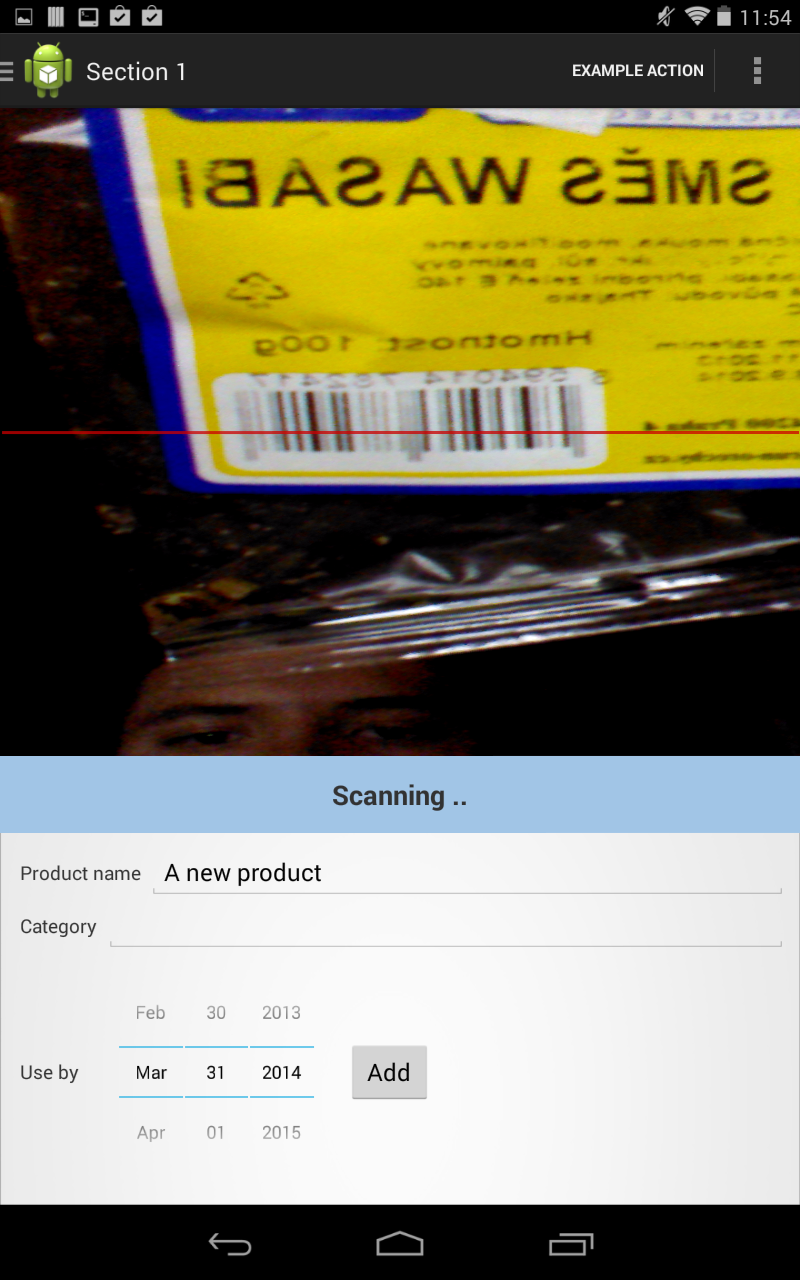
\includegraphics[scale=0.3]{screenshots/scan_prototype.png}
  \caption{Prototyp snímaní čárových kódů}
  \label{fig:ScanPrototype}
\end{figure}

\clearpage

\section{Případy užití}

Výše uvedené funkční požadavky se přimo promítají do případů užití. Tento diagram slouží pří návrhu UI i jako scénáře pro uživatelské testování, které ověří, zda daný návrh je pro uživatele dostatečne jednoduchý a zda-li je uživatel schopen v aplikaci dosáhnout všech daných cílu.

Inventář a vyhledání potraviny jsou základnami, ze kterých se dále odvíjejí ostatní činnosti. Jednotlivé případy vystihují přesně ty činnosti, které bude uživatel provádět během používání aplikace.

Při vytváření tohoto diagramu byl dán veliký důraz na nejčastější činnosti uživatele, které lze očekávat. V závěru práce dojde ke zhodnocení zde navrhnutých scénářů a přípádné návrhy na změnu do budoucnosti.

\begin{figure}[H]
  \centering
  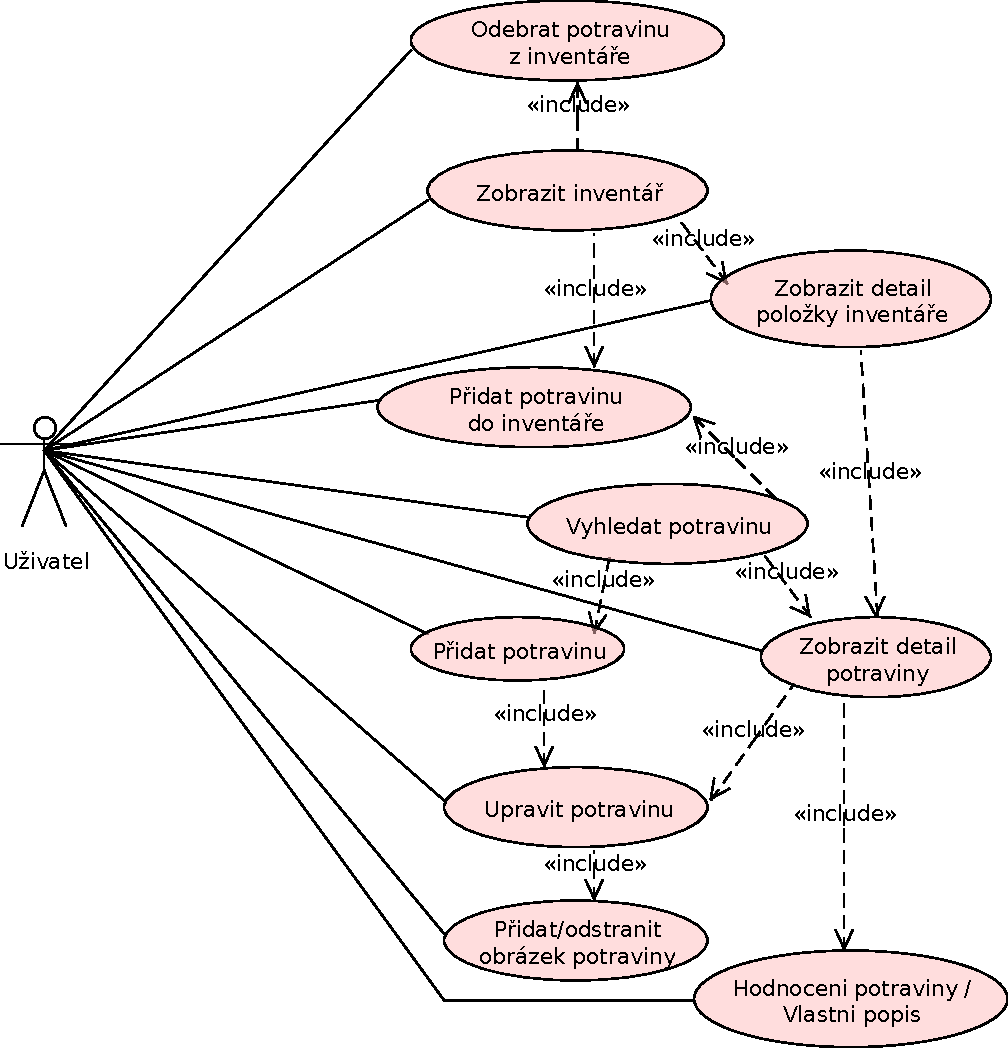
\includegraphics[scale=0.75]{diagrams/use_case}
  \caption{Diagram případů užití}
  \label{fig:UseCase}
\end{figure}

\chapter{Návrh}

Kapitola návrh poskytne soubor informací k následné implementaci. Požadavky sepsány v kapitole Analýza budou pevně diktovat jeho obsah. Struktura návrhu se týka návrhu architektury, doménového modelu, databázového modelu, bussiness modelu, class diagramu a popis komunikačního protokolu.

\section{Architektura}

Vzhledem nutnosti použít pro mobilní aplikaci server bude nejvhodnější model architektury klient - server. Tento model vyžaduje specifikovat komunikaci mezi obouma stranami a dále při vhodném navrhnutí lze uvažovat i o klientech pro více platforem. Vhodná platforma pro jiný typ aplikace by mohla být webová aplikace, která by zpřístupňovala aplikaci na všech ostatních platformách skrze webový prohlížeč. Touto cestou by však nebylo možné uživatele jednoduše upozorňovat o trvanlivosti přímo z webové stránky i v době, kdy uživatel stránku nepoužívá.

\subsection{Klient}

Z nefunkčního požadavku OS Android vyplývá nutnost implementovat aplikaci s pomocí jeho SDK. Existují multiplatformní SDK nabízející bežné API, avšak nutnost vytváření upozornění a snímaní čárových kódů je čistě specifická záležitost pro kažou platformu zvlášť. Tuto možnost autor předpokládá jako časově náročnou, proto se tato práce soustředí pouze na Android SDK.

\subsection{Server}

Jako jeden z hlavních požadavků na server je jeho malý paměťový otisk. Nabízí se spousta různých variant, jak tohoto cíle dosáhnout. Jelikož předměty prvního ročníku autorova studia obsahovali především algoritmizace v jazycích C/C++ a obor softwarového inženýrství si vyžádal předmět efektivních algoritmů, byla jako vhodná varianta serveru jeho implementace v jazyce C++. Bližší detaily jeho návrhu budou priblíženy dále.

\section{Doménový model}

Na obrázku doménovém modelu ~\ref{fig:ScanPrototype} lze spatřit vztahy mezi všemi entitami, jejichž význam zde bude vysvětlen.

\subsection{Category}
Category poskytuje kategorizaci potravin. Tato entita je připravena pro budoucí rozšíření vyhledávání, v rámci této práce je informace o kategorii pouze shromažďována. 

\subsection{Edit}
Každá editace potraviny tvoří záznam entity Edit, ve které se nachází informace kdo, kdy a co upravil. Tato informace poté může sloužit k blokování škodlivých uživatelů.

\subsection{Food}
Entita food popisuje potravinu.

\subsection{Image}
Každá potravina může nabýt předem nespecifikované množství obrázků od uživatelů.

\subsection{Inventory}
Položka inventáře spojující uživatele a potravinu, která zároveň určuje datum spotřeby. Při přidání několika instancí potraviny do inventáře najednou se vždy přidá stejný počet záznamů této entity.

\subsection{Review}
Jednoduché hodnocení potraviny od 0 do 5 s volitelným textem recenze uživatele. Každý uživatel může nabýt nejvíce 1 hodnocení.

\subsection{User}
Entita uživatele, uchovávající pouze uživatelské jméno. Tuto entitu bude nutné v budoucnu rozšířit o příslušné vlastnosti pokud bude třeba uživatelská data více zabezpečit.

\subsection{Vendor}
Výrobce je specifikován jako samostatná entita, v budoucnu lze také použít pro filtrování vyhledávání stejně jako je tomu u kategorie.

\begin{figure}[H]
  \centering
  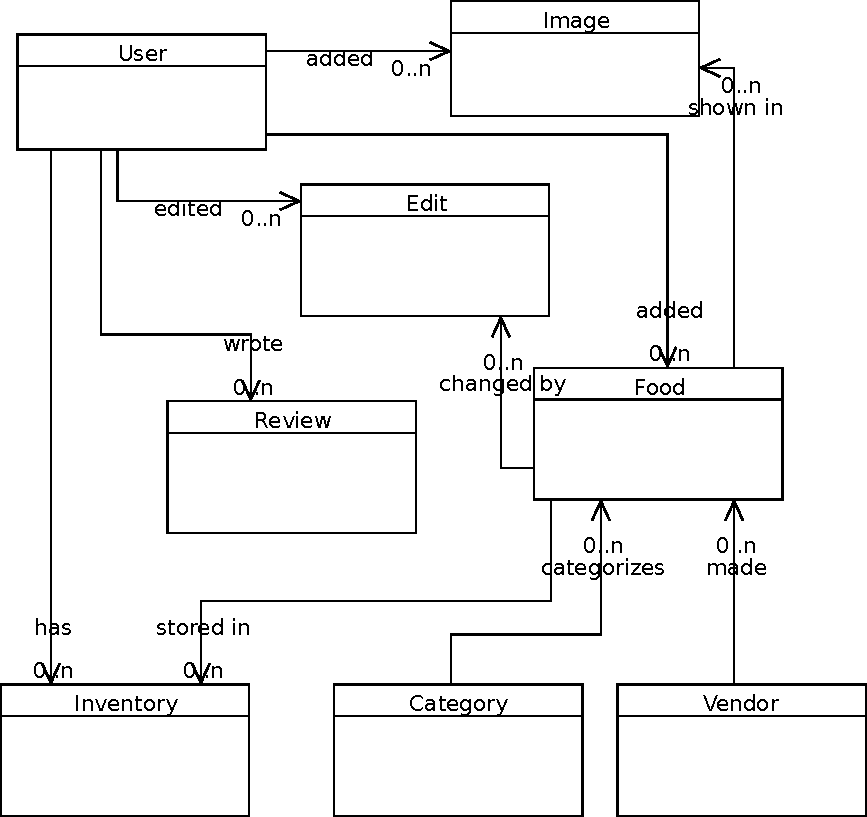
\includegraphics[scale=0.75]{diagrams/model}
  \caption{Doménový model}
  \label{fig:DomainModel}
\end{figure}

\section{Databázový model}

\begin{figure}[H]
  \centering
  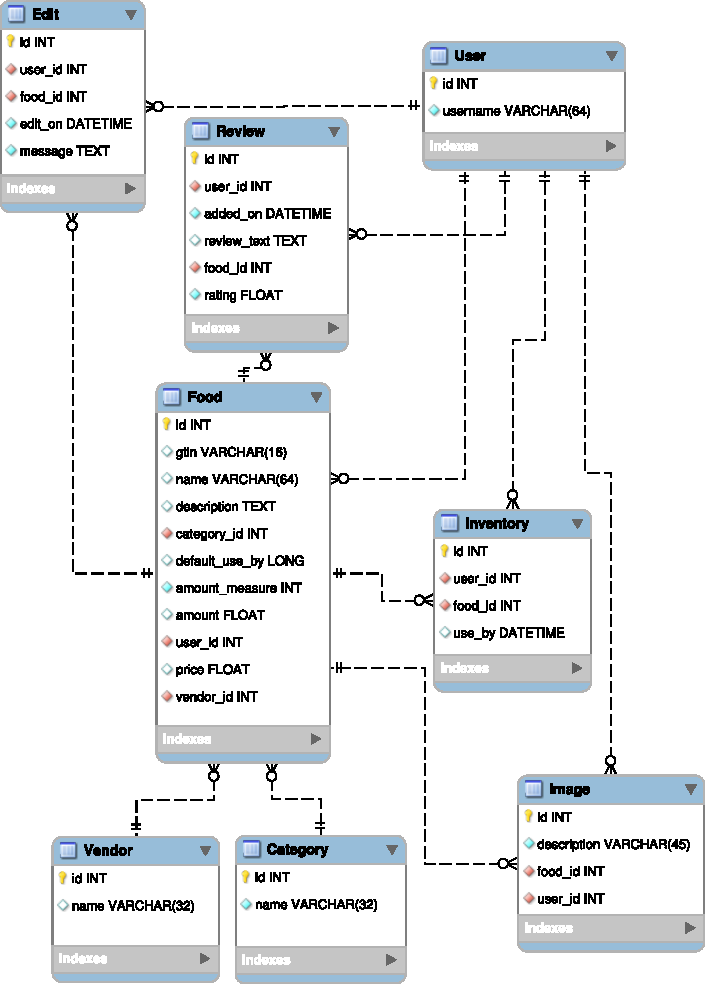
\includegraphics[scale=1.20]{diagrams/relational_model}
  \caption{Relační model}
  \label{fig:RelationalModel}
\end{figure}


\section{Komunikační formát a protokol}

Z důvodu zvolené architektury je nutné specifikovat protokol, jakým budou mezi sebou komunikovat klient a server. Android SDK diktuje pro mobilního klienta použití jazyku Java, který sice lze nahradit pomocí C/C++, toho se však doporučuje jen v aplikací či knihovnách s potřebou vysokého výkonu nebo přístupu k hardware ~\cite{android_ndk}. Tato odlišnost vyžaduje použít platformě nezávislý protokol na bázi například textu.

\subsection{XML}

Mnoho protokolů využíva ke komunikaci textový formát v XML. Tento formát je podobný HTML, je platformě nezávislý a široce podporován. V C/C++ ho implementují různé knihovny, které jsou dostupné jako svobodný software. Protokol však nevyžívá datový prostor dostatečně efektivně, jak bude popsáno dále.

\subsection{JSON}

Jako další textový formát umožňující platformově nezávislý přenos dat je JSON. Je to velice populární formát používaný široce ve webových technologiích a jeho použití je také velmi jednoduché. Formát vychází z JavaScriptové notace a lze ho s bezpečnostními opatřeními načíst jako samotný zdrojový kód JavaScriptu. Výhodou formátu JSON je jeho kompaktnost oproti formátu XML, čímž dojde ke snížení přenášeného množství dat a přesto se zachová textový formát dat.

\subsection{Porovnání a zvolení formátu}

Oba formáty jsou přímo podporovány v Android API a tak jsou vhodnými kandidáty. Od obou formátu jsou k dispozici různé kompaktnější verze, které ještě více data zhušťují nebo využívají jiné kompresní algoritmy pro snížení velikosti jejich dat. Využití takovýchto vylepšení je však omezující jeho podporou různých prostředí a neumožňují lidsky čitelný formát, který je vhodný pro vývoj a odhalování chyb.

Různé knihovny implementují tyto formáty i do C++, které jejich podporu ve standardních knihovnách neobsahuje. Jelikož jediný patrný rozdíl je ve větší kompaktnosti, byl zvolen JSON jako formát protokolu pro tuto aplikaci.

\subsection{Struktura protokolu}

Protokol budou tvořit zprávy, které budou mít pevný tvar. Kvůli možnosti budoucího vylepšení protokolu a jednoduchosti jeho načtení ze síťového proudu je vhodné poslat přesný počet bytů každé zprávy vepvně daném pořadí. Zpráva bude mít teoreticky neomezenou velikost, avšak server bude mít možnost tuto velikost omezit kvůli zabránění zahlcení serveru jednoduchým útokem, který by zaplnil celou dostupnou pamět a způsobil pád serveru. Maximální velikost zprávy bude možné nastavit v serveru a bude také hodnota, která s dalšími vlastnostmi určí maximální množství uživatelů, který je server schopen v extrémním případě obsloužit.

Komunikaci budou tvořit zprávy přenesené v přesném pořadí jako:

\begin{itemize}
  \item{4 byty určující celé číslo N v Big Endian pořadí, stejné jako Network Byte Order}
  \item{N bytů textové UTF-8 zprávy}
\end{itemize}

Zprávy budou mít dále již v JSON formátu strukturu:
\begin{lstlisting}
{
  "header" : "NazevZpravy",
  "content" :
    {
      .. dalsi obsah zpravy ..
    }
}
\end{lstlisting}

\begin{itemize}
  \item{položka header určuje název zprávy, který bude popsán dále}
  \item{položka content obsahuje položky určité zprávy}
\end{itemize}

Zprávy budou mít povahu požadavku a odpovědi na něj. Klient bude posílat serveru požadavky a ten mu na ně příslušně odpovídat. Neznámé zprávy způsobí ukončení komunikace.

Jednotlivé zprávy byly navrženy již s ohledem na funkce uživatelského rozhraní. Tyto zprávy budou dále popsány, jejich pevnou strukturu však bude možné zjistit ze zdrojového kódu, neboť rozsah této práce takovouto specifikaci neumožňuje. Zprávy kromě poslední KeepAlive jsou dvojice Request a Respond, např. pro zprávu Login to je LoginRequest a LoginResponse.

\begin{itemize}
  \item{\textbf{Login} - přihlásí uživatele pod jménem (e-mailem) a vrátí odpověď jako boolean, zda-li tak proběhlo}
  \item{\textbf{GetInventory} - vyhledá a vrátí množinu položek inventáře podle zadaného jména nebo kódu GTIN}
  \item{\textbf{GetFoodDetail} - vratí veškeré detaily potraviny}
  \item{\textbf{GetFoodItem} - vyhledá vrátí množinu potravin podle jména nebo GTIN kódu}
  \item{\textbf{EditInventory} - upraví položku inventáře}
  \item{\textbf{DeleteInventory} - smaže položku inventáře}
  \item{\textbf{EditFood} - upraví detail potraviny}
  \item{\textbf{GetFoodBase} - vrátí podklady k zadání potraviny: výrobce a kategorie}
  \item{\textbf{AddImage} - nahraje nový obrázek potraviny}
  \item{\textbf{DeleteImage} - smaže zadaný obrázek potraviny}
  \item{\textbf{SetUserReview} - nastaví nebo smaže uživatelovu recenzi}
  \item{\textbf{KeepAlive} - příkaz udržující spojení po dobu od posledního}
\end{itemize}

\begin{conclusion}
	%sem napište závěr Vaší práce
\end{conclusion}

\bibliographystyle{csn690}
\bibliography{mybibliographyfile}

\appendix

\chapter{Seznam použitých zkratek}
% \printglossaries
\begin{description}
	\item[API] Application Programming Interface
	\item[HTML] HyperText Markup Language
	\item[JSON] JavaScript Object Notation
	\item[NDK] Native Development Kit
	\item[OS] Operační systém
	\item[SDK] Software Development Kit
	\item[VM] Virtual Machine
	\item[XML] Extensible Markup Language
\end{description}



% % % % % % % % % % % % % % % % % % % % % % % % % % % % 
% % Tuto kapitolu z výsledné práce ODSTRAŇTE.
% % % % % % % % % % % % % % % % % % % % % % % % % % % % 
% 
% \chapter{Návod k~použití této šablony}
% 
% Tento dokument slouží jako základ pro napsání závěrečné práce na Fakultě informačních technologií ČVUT v~Praze.
% 
% \section{Výběr základu}
% 
% Vyberte si šablonu podle druhu práce (bakalářská, diplomová), jazyka (čeština, angličtina) a kódování (ASCII, \mbox{UTF-8}, \mbox{ISO-8859-2} neboli latin2 a nebo \mbox{Windows-1250}). 
% 
% V~české variantě naleznete šablony v~souborech pojmenovaných ve formátu práce\_kódování.tex. Typ může být:
% \begin{description}
% 	\item[BP] bakalářská práce,
% 	\item[DP] diplomová (magisterská) práce.
% \end{description}
% Kódování, ve kterém chcete psát, může být:
% \begin{description}
% 	\item[UTF-8] kódování Unicode,
% 	\item[ISO-8859-2] latin2,
% 	\item[Windows-1250] znaková sada 1250 Windows.
% \end{description}
% V~případě nejistoty ohledně kódování doporučujeme následující postup:
% \begin{enumerate}
% 	\item Otevřete šablony pro kódování UTF-8 v~editoru prostého textu, který chcete pro psaní práce použít -- pokud můžete texty s~diakritikou normálně přečíst, použijte tuto šablonu.
% 	\item V~opačném případě postupujte dále podle toho, jaký operační systém používáte:
% 	\begin{itemize}
% 		\item v~případě Windows použijte šablonu pro kódování \mbox{Windows-1250},
% 		\item jinak zkuste použít šablonu pro kódování \mbox{ISO-8859-2}.
% 	\end{itemize}
% \end{enumerate}
% 
% 
% V~anglické variantě jsou šablony pojmenované podle typu práce, možnosti jsou:
% \begin{description}
% 	\item[bachelors] bakalářská práce,
% 	\item[masters] diplomová (magisterská) práce.
% \end{description}
% 
% \section{Použití šablony}
% 
% Šablona je určena pro zpracování systémem \LaTeXe{}. Text je možné psát v~textovém editoru jako prostý text, lze však také využít specializovaný editor pro \LaTeX{}, např. Kile.
% 
% Pro získání tisknutelného výstupu z~takto vytvořeného souboru použijte příkaz \verb|pdflatex|, kterému předáte cestu k~souboru jako parametr. Vhodný editor pro \LaTeX{} toto udělá za Vás. \verb|pdfcslatex| ani \verb|cslatex| \emph{nebudou} s~těmito šablonami fungovat.
% 
% Více informací o~použití systému \LaTeX{} najdete např. v~\cite{wikilatex}.
% 
% \subsection{Typografie}
% 
% Při psaní dodržujte typografické konvence zvoleného jazyka. České \uv{uvozovky} zapisujte použitím příkazu \verb|\uv|, kterému v~parametru předáte text, jenž má být v~uvozovkách. Anglické otevírací uvozovky se v~\LaTeX{}u zadávají jako dva zpětné apostrofy, uzavírací uvozovky jako dva apostrofy. Často chybně uváděný symbol "{} (palce) nemá s~uvozovkami nic společného.
% 
% Dále je třeba zabránit zalomení řádky mezi některými slovy, v~češtině např. za jednopísmennými předložkami a spojkami (vyjma \uv{a}). To docílíte vložením pružné nezalomitelné mezery -- znakem \texttt{\textasciitilde}. V~tomto případě to není třeba dělat ručně, lze použít program \verb|vlna|.
% 
% Více o~typografii viz \cite{kobltypo}.
% 
% \subsection{Obrázky}
% 
% Pro umožnění vkládání obrázků je vhodné použít balíček \verb|graphicx|, samotné vložení se provede příkazem \verb|\includegraphics|. Takto je možné vkládat obrázky ve formátu PDF, PNG a JPEG jestliže používáte pdf\LaTeX{} nebo ve formátu EPS jestliže používáte \LaTeX{}. Doporučujeme preferovat vektorové obrázky před rastrovými (vyjma fotografií).
% 
% \subsubsection{Získání vhodného formátu}
% 
% Pro získání vektorových formátů PDF nebo EPS z~jiných lze použít některý z~vektorových grafických editorů. Pro převod rastrového obrázku na vektorový lze použít rasterizaci, kterou mnohé editory zvládají (např. Inkscape). Pro konverze lze použít též nástroje pro dávkové zpracování běžně dodávané s~\LaTeX{}em, např. \verb|epstopdf|.
% 
% \subsubsection{Plovoucí prostředí}
% 
% Příkazem \verb|\includegraphics| lze obrázky vkládat přímo, doporučujeme však použít plovoucí prostředí, konkrétně \verb|figure|. Například obrázek \ref{fig:float} byl vložen tímto způsobem. Vůbec přitom nevadí, když je obrázek umístěn jinde, než bylo původně zamýšleno -- je tomu tak hlavně kvůli dodržení typografických konvencí. Namísto vynucování konkrétní pozice obrázku doporučujeme používat odkazování z~textu (dvojice příkazů \verb|\label| a \verb|\ref|).
% 
% \begin{figure}\centering
% 	
\includegraphics[width=0.5\textwidth, angle=30]{cvut-logo-bw}
% 	\caption[Příklad obrázku]{Ukázkový obrázek v~plovoucím prostředí}\label{fig:float}
% \end{figure}
% 
% \subsubsection{Verze obrázků}
% 
% % Gnuplot BW i barevně
% Může se hodit mít více verzí stejného obrázku, např. pro barevný či černobílý tisk a nebo pro prezentaci. S~pomocí některých nástrojů na generování grafiky je to snadné.
% 
% Máte-li například graf vytvořený v programu Gnuplot, můžete jeho černobílou variantu (viz obr. \ref{fig:gnuplot-bw}) vytvořit parametrem \verb|monochrome dashed| příkazu \verb|set term|. Barevnou variantu (viz obr. \ref{fig:gnuplot-col}) vhodnou na prezentace lze vytvořit parametrem \verb|colour solid|.
% 
% \begin{figure}\centering
% 	\includegraphics{gnuplot-bw}
% 	\caption{Černobílá varianta obrázku generovaného programem Gnuplot}\label{fig:gnuplot-bw}
% \end{figure}
% 
% \begin{figure}\centering
% 	\includegraphics{gnuplot-col}
% 	\caption{Barevná varianta obrázku generovaného programem Gnuplot}\label{fig:gnuplot-col}
% \end{figure}
% 
% 
% \subsection{Tabulky}
% 
% Tabulky lze zadávat různě, např. v~prostředí \verb|tabular|, avšak pro jejich vkládání platí to samé, co pro obrázky -- použijte plovoucí prostředí, v~tomto případě \verb|table|. Například tabulka \ref{tab:matematika} byla vložena tímto způsobem.
% 
% \begin{table}\centering
% 	\caption[Příklad tabulky]{Zadávání matematiky}\label{tab:matematika}
% 	\begin{tabular}{|l|l|c|c|}\hline
% 		Typ		& Prostředí		& \LaTeX{}ovská zkratka	& \TeX{}ovská zkratka	\tabularnewline \hline \hline
% 		Text		& \verb|math|		& \verb|\(...\)|	& \verb|$...$|		\tabularnewline \hline
% 		Displayed	& \verb|displaymath|	& \verb|\[...\]|	& \verb|$$...$$|	\tabularnewline \hline
% 	\end{tabular}
% \end{table}
% 
% % % % % % % % % % % % % % % % % % % % % % % % % % % % 

\chapter{Obsah přiloženého CD}

%upravte podle skutecnosti

\begin{figure}
	\dirtree{%
		.1 readme.txt\DTcomment{stručný popis obsahu CD}.
		.1 exe\DTcomment{adresář se spustitelnou formou implementace}.
		.1 src.
		.2 impl\DTcomment{zdrojové kódy implementace}.
		.2 thesis\DTcomment{zdrojová forma práce ve formátu \LaTeX{}}.
		.1 text\DTcomment{text práce}.
		.2 thesis.pdf\DTcomment{text práce ve formátu PDF}.
		.2 thesis.ps\DTcomment{text práce ve formátu PS}.
	}
\end{figure}

\end{document}
